\subsection{Calculation of current activity}
Given radioactive source is Cs-137 haing activity 3.7 MBq on September 2022. So the current activity can be calculated using the formula:
\begin{equation}
    A = A_0 e^{-\lambda t}
\end{equation}
Where, $A_0$ is the initial activity, $\lambda$ is the decay constant and $t$ is the time elapsed. The decay constant can be calculated using the formula:  
\begin{equation}
    \lambda = \frac{\ln(2)}{T_{1/2}}
\end{equation}
Where $T_{1/2}$ is the half-life of the isotope. For Cs-137, $T_{1/2} = 30.0$ years.
Calculating $\lambda$:
\begin{equation}
    \lambda = \frac{\ln(2)}{30.0} = 0.0231 \text{ year}^{-1}
\end{equation}
Calculating the time elapsed from September 2022 to February 2026:
\begin{equation}
    t = 3.33 \text{ years}
\end{equation}
Now, calculating the current activity:
\begin{equation}
    A = 3.7 \text{ MBq} \times e^{-0.0231 \times 3.33} = 3.7 \text{ MBq} \times e^{-0.076923} = 3.7 \text{ MBq} \times 0.9258 = 3.42 \text{ MBq}
\end{equation}
So, the current activity of the Cs-137 source is approximately 3.418 MBq or 0.0924 mCi.
\subsection{True dose rate (R)}
The true dose rate can be calculated using the formula:
\begin{equation}
    R = \frac{A \cdot \Gamma}{d^2}
\end{equation}
Where, $A$ is the activity of the source, $\Gamma$ is the specific gamma ray constant for Cs-137, and $d$ is the distance from the source. The specific gamma ray constant for Cs-137 is approximately 3.2267 R cm$^2$ / mCi h. Converting the activity from MBq to Ci:
\begin{equation}
    A = 3.418 \text{ MBq} = 0.0924 \text{ mCi}
\end{equation}
Now, calculating the true dose rate at a distance of 50 centimeter:
\begin{equation}
    R = \frac{0.0924 \text{ mCi} \times 3.2267 \text{ R cm}^2/\text{mCi h}}{(50 \text{ cm})^2} = 118.95 \text{$\mu$R/h}    
\end{equation}

\subsection{Response for Fluke 451 P}
Place the fluke 451 P at a distance of 50 cm from the source and measure the dose rate. Different orientations of the detector can be used to measure the dose rate and compare it with the true dose rate calculated above. 
\begin{figure}[H]
    \centering
    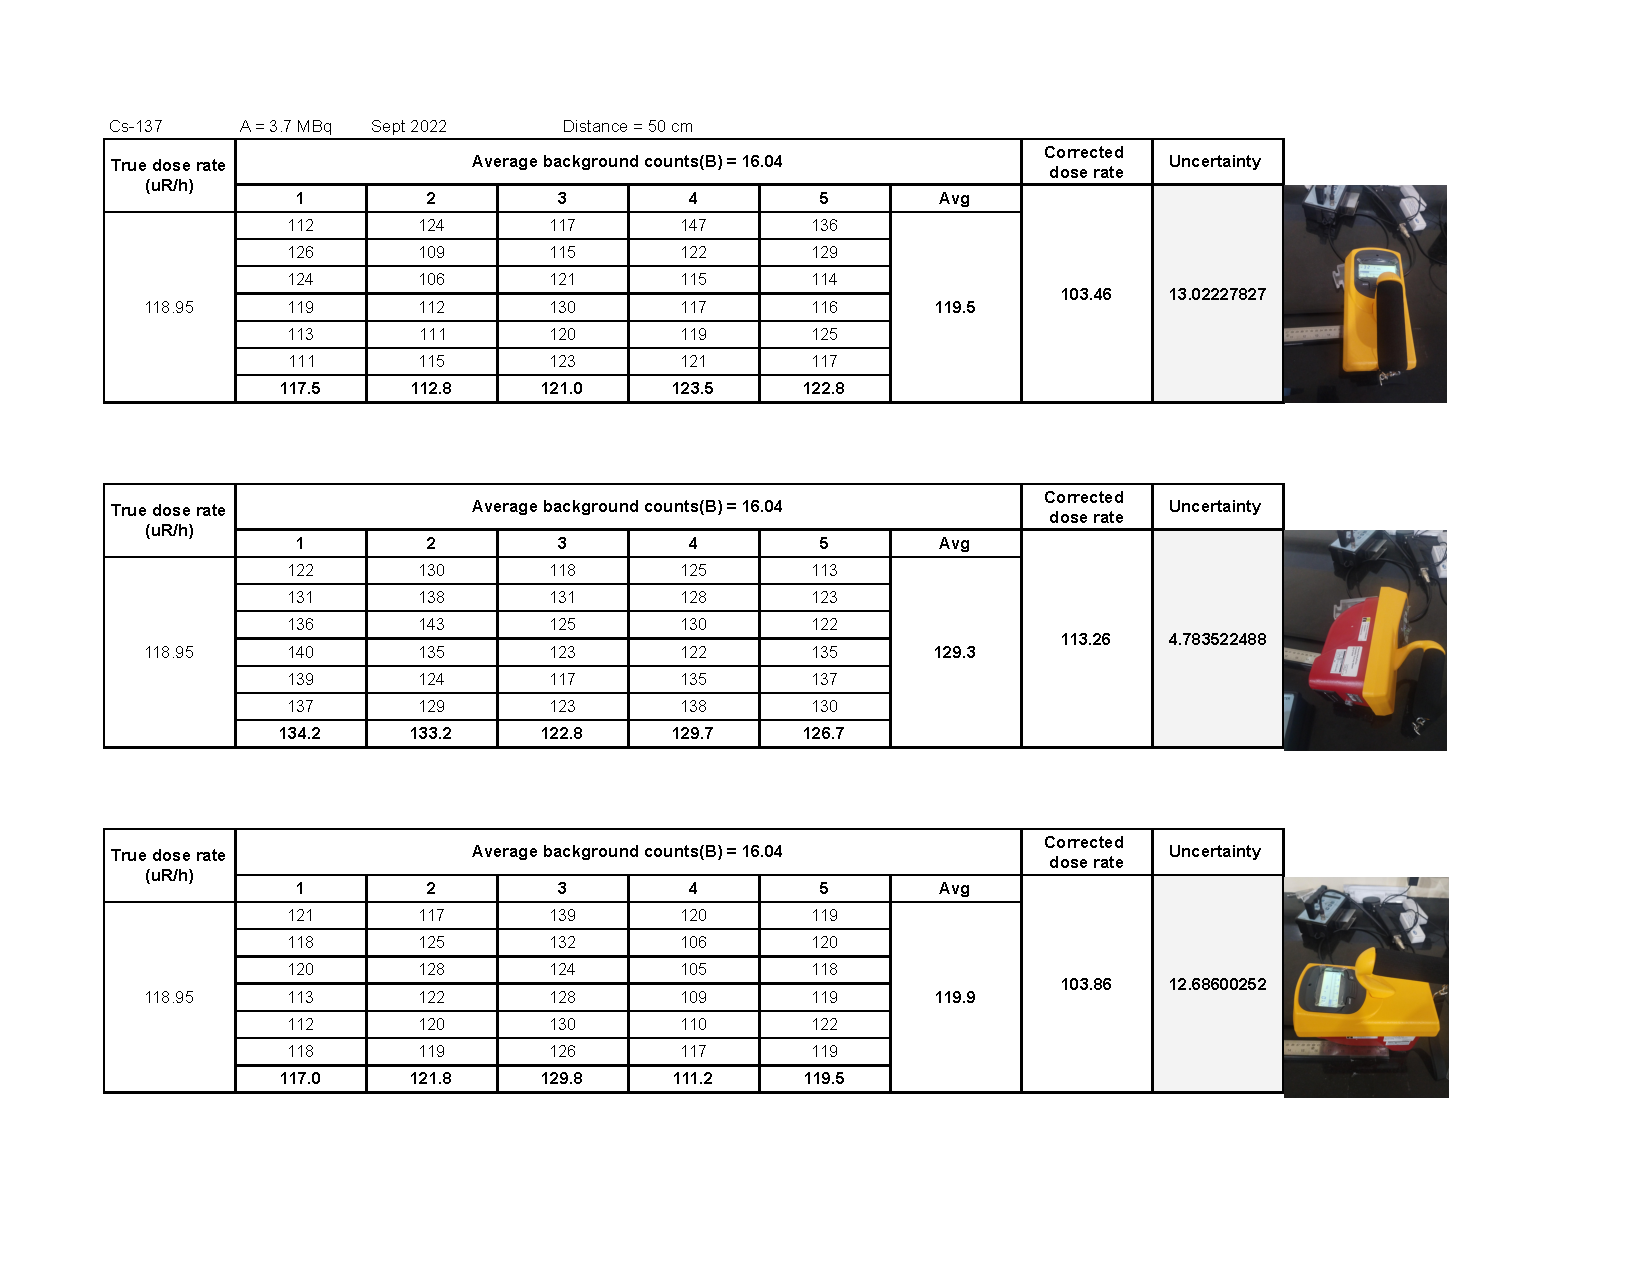
\includegraphics[width=\textwidth]{Figures/Experimental data/Validation of Calibration - Fluke.pdf}
\end{figure}
It is canbe seen that 2nd Orientation of the detector gives the closest reading to the true dose rate calculated above.
\subsection{Response for Survey Meter}
\begin{figure}[H]
    \centering
    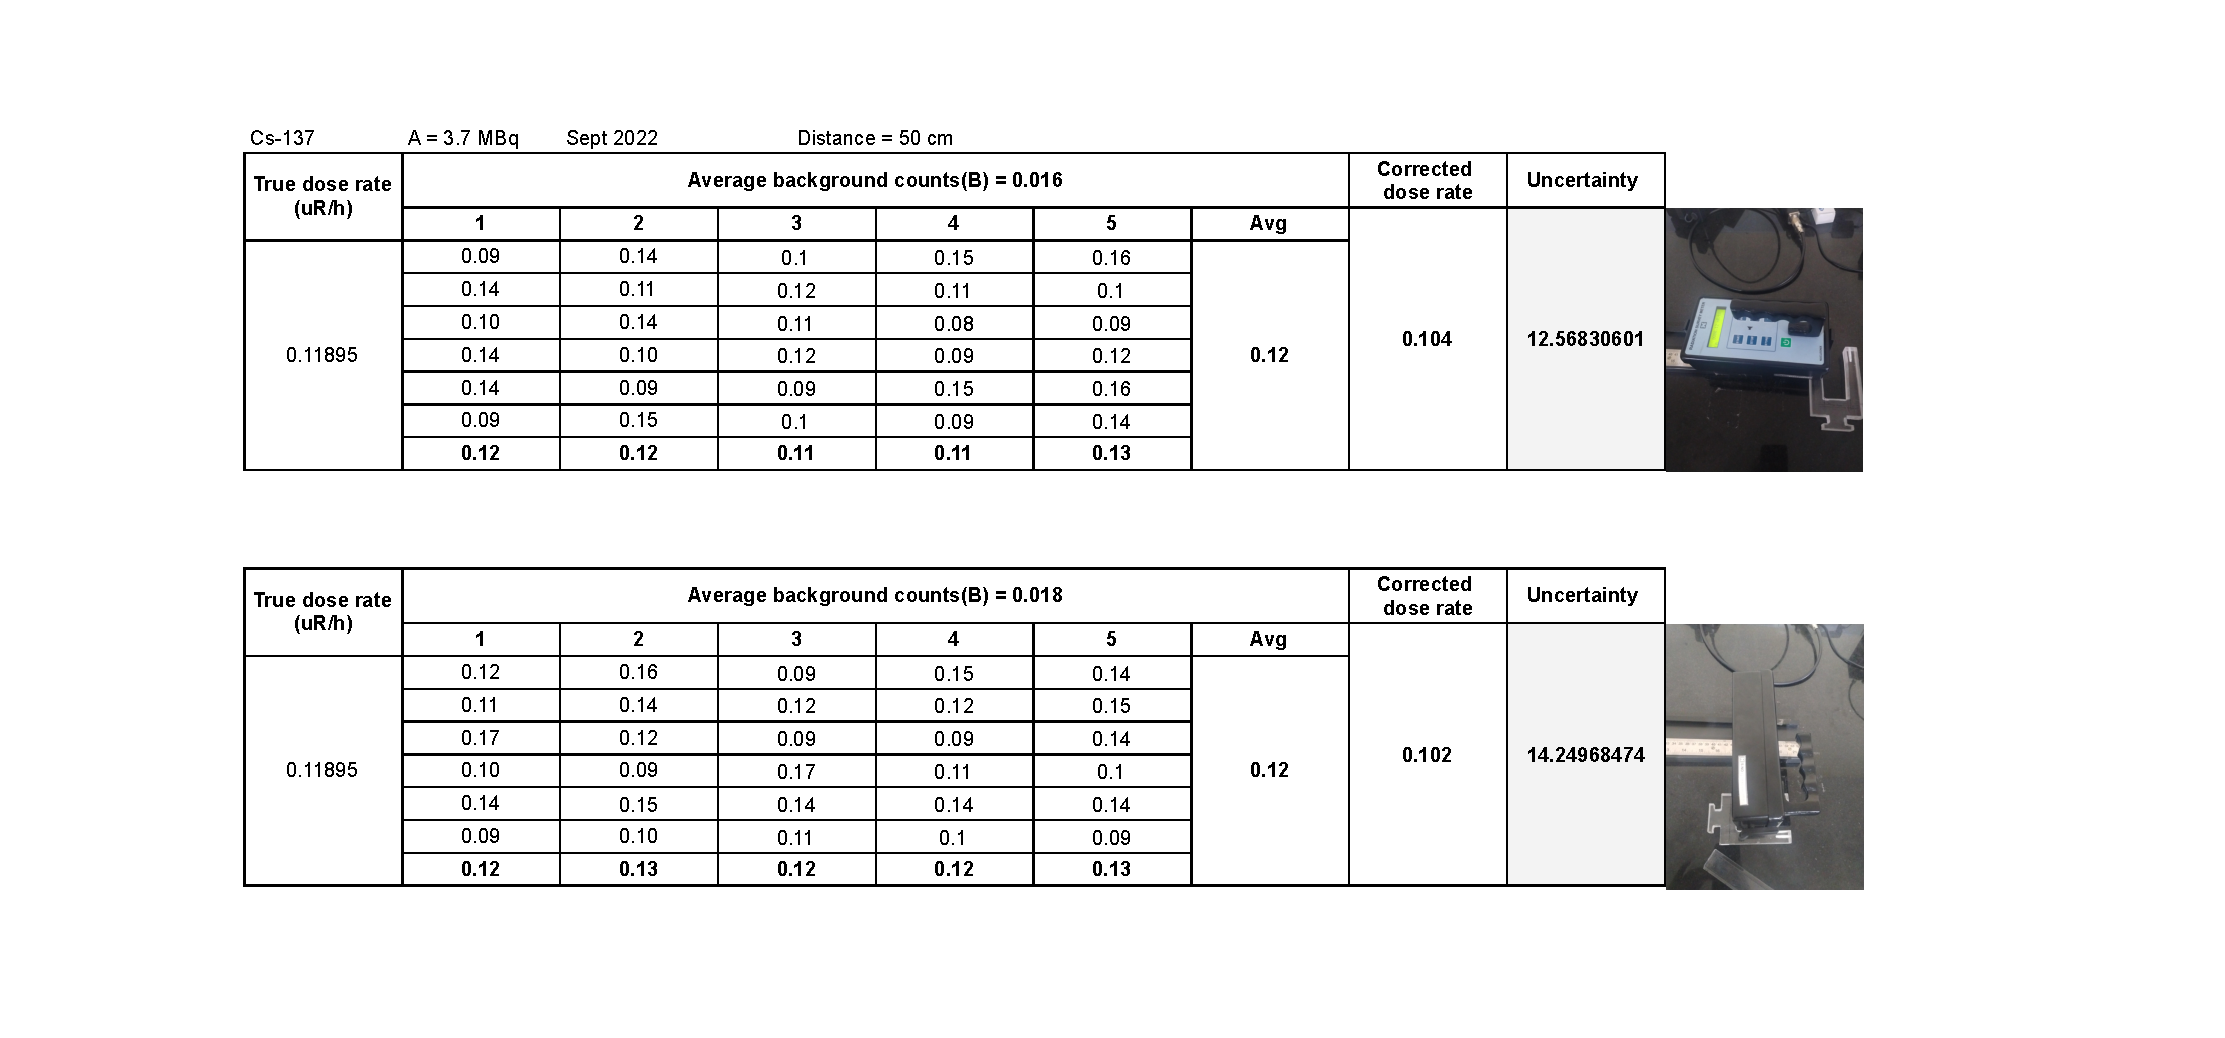
\includegraphics[width=\textwidth]{Figures/Experimental data/Validation of Calibration - Survey Meter.pdf}
\end{figure}

\subsection{Response for Contamination Monitor}
\begin{figure}[H]
    \centering
    \includegraphics[width=\textwidth]{Figures/Experimental data/Validation of Calibration - Contamination Monitor.pdf}
\end{figure}

\subsection{True dose(D)}
The true dose can be calculated using the formula:
\begin{equation}    D = R \cdot t
\end{equation}
Where, $R$ is the true dose rate in Sv/min and $t$ is the time of exposure. Converting the true dose rate from $\mu$R/h to Sv/min for 10 cm distance:
\begin{equation}
    R = 26.13 \text{ $\mu$Sv/hr} = 0.4355 \text{ $\mu$Sv/min}
\end{equation}
Now, calculating the true dose for 10 minutes of exposure:
\begin{equation}    D = 0.4355 \text{ $\mu$Sv/min} \times 10 \text{ min} = 4.355 \text{ $\mu$Sv}
\end{equation}
\begin{equation}    D = 0.4355 \text{ $\mu$Sv/min} \times 20 \text{ min} = 8.71 \text{ $\mu$Sv}
\end{equation}
\subsection{Micro Digital Pocket Dosimeter}
\begin{figure}[H]
    \centering
    \includegraphics[width=\textwidth]{Figures/Experimental data/Validation of Calibration - Pocket Dosimeter.pdf}
\end{figure}